\documentclass{article}
\usepackage[pdftex]{graphicx}
\usepackage{listings}
\usepackage{xcolor}
\lstset{basicstyle=\ttfamily,
  showstringspaces=false,
  commentstyle=\color{red},
  keywordstyle=\color{blue}
}
\begin{document}

\author{Jon Robison}
\title{CS595 Assignment 4}
\maketitle

Q1. From your list of 1000 links, choose 100 and extract all of the links from
those 100 pages to other pages...Upload these 100 files to github. \\
Large collection of files included in results directory \\
See Appendix A for download program
\\*

Q2. Using these 100 files, create a single GraphViz ``dot'' file of the resulting
graph \\
See Appendix B for script to produce plot \\
See Appendix C for dot file
\\*

Q3. Download and install Gephi...Load the dot file created in \#2 and use Gephi
to:\\
- visualize the graph (you'll have to turn on labels)\\
- calculate HITS and PageRank\\
- avg degree\\
- network diameter\\
- connected components\\
\vfill
\graphicspath{{q3/}}
\begin{figure}
  \centering
  \caption{Graph with labels}
  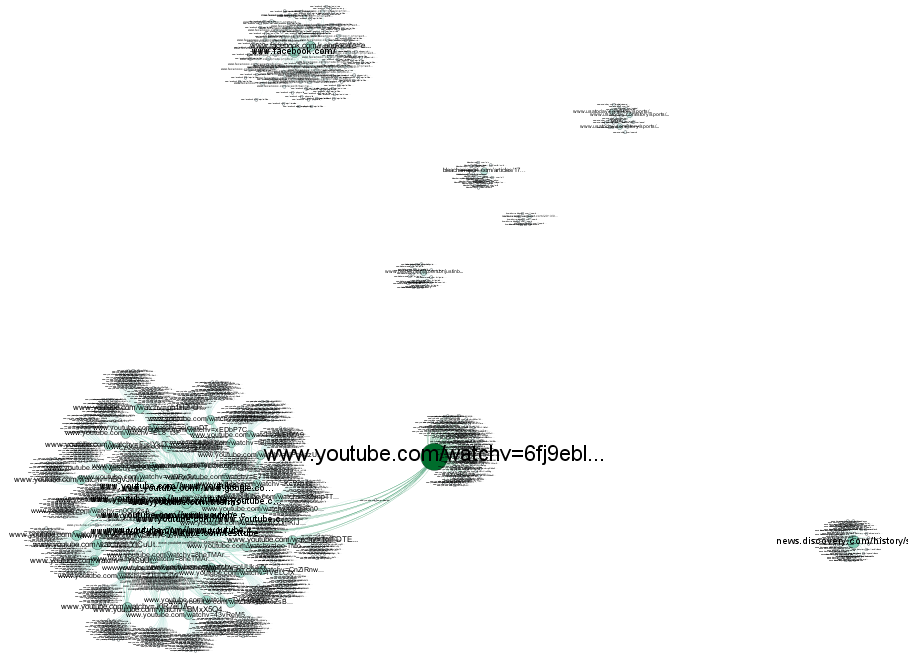
\includegraphics[scale=.35]{graph.png}
\end{figure}
\begin{figure}
  \centering
  \caption{Graph without labels}
  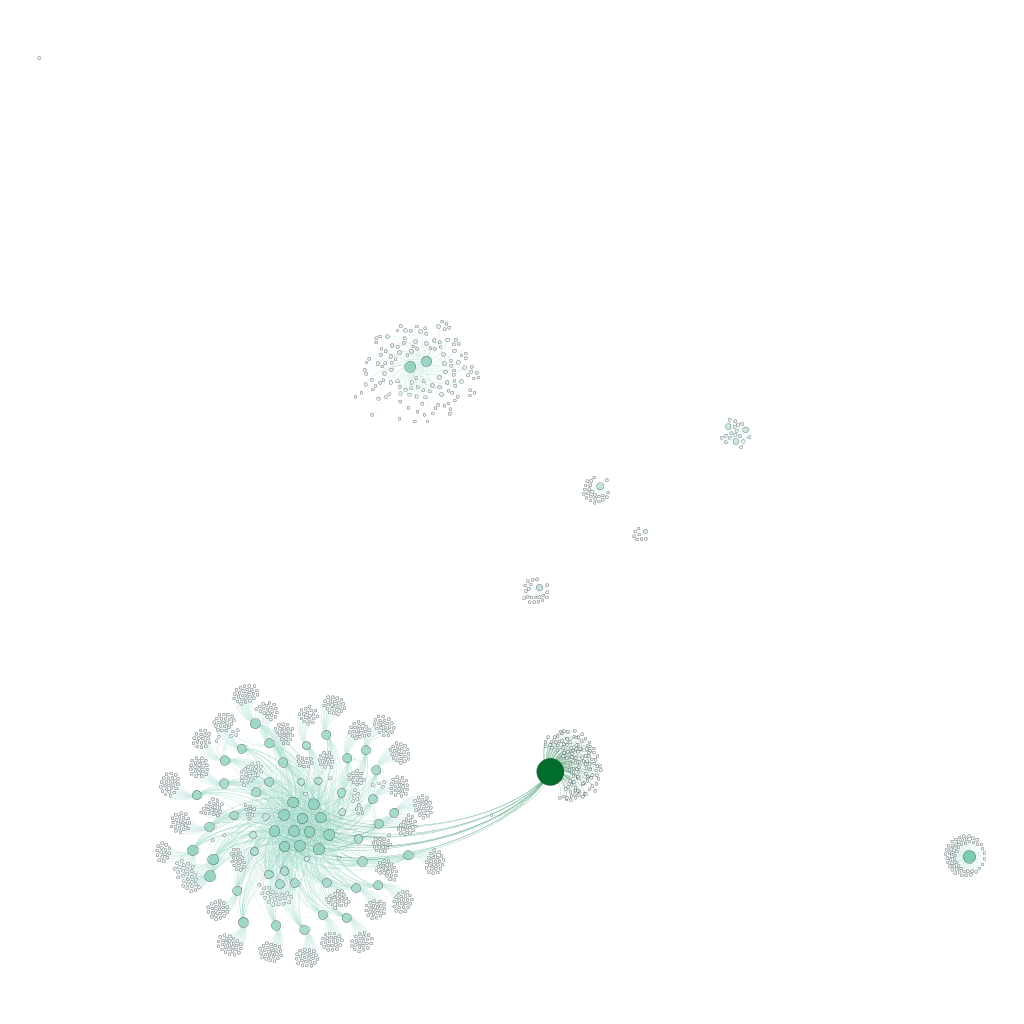
\includegraphics[scale=.35]{graphNoLabels.png}
\end{figure}
\graphicspath{{q3/avgDegree/}}
\begin{figure}
  \centering
  \caption{Degree distribution}
  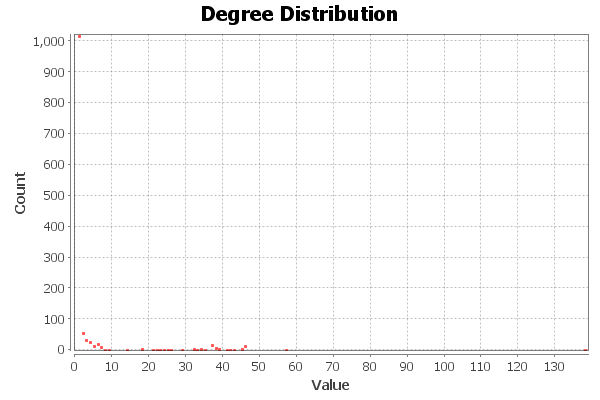
\includegraphics[scale=.5]{degree-distribution.png}
\end{figure}
\begin{figure}
  \centering
  \caption{In-degree distribution}
  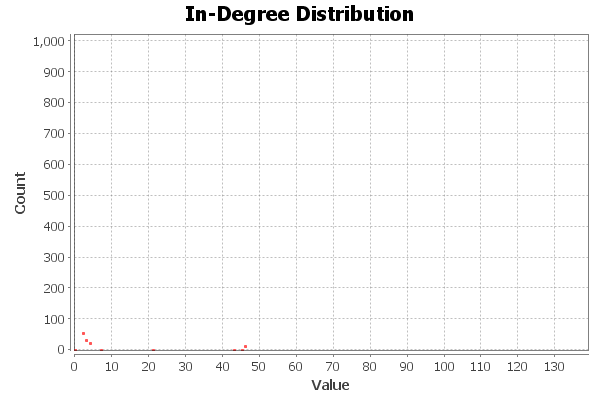
\includegraphics[scale=.5]{indegree-distribution.png}
\end{figure}
\begin{figure}
  \centering
  \caption{Out-degree distribution}
  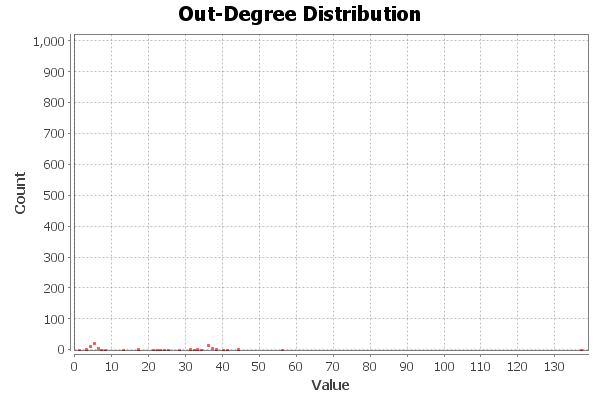
\includegraphics[scale=.5]{outdegree-distribution.png}
\end{figure}
\graphicspath{{q3/connected/}}
\begin{figure}
  \centering
  \caption{Connected distribution}
  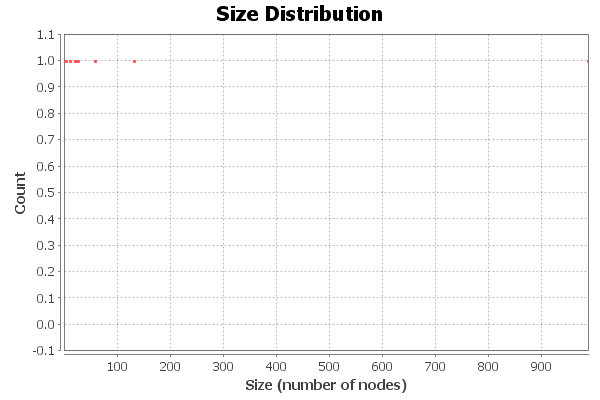
\includegraphics[scale=.5]{cc-size-distribution.png}
\end{figure}
\graphicspath{{q3/diameter/}}
\begin{figure}
  \centering
  \caption{Closeness centrality distribution}
  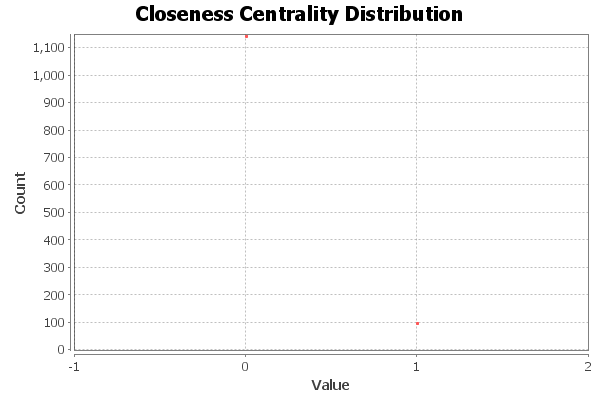
\includegraphics[scale=.5]{ClosenessCentralityDistribution.png}
\end{figure}
\begin{figure}
  \centering
  \caption{Betweenness centrality distribution}
  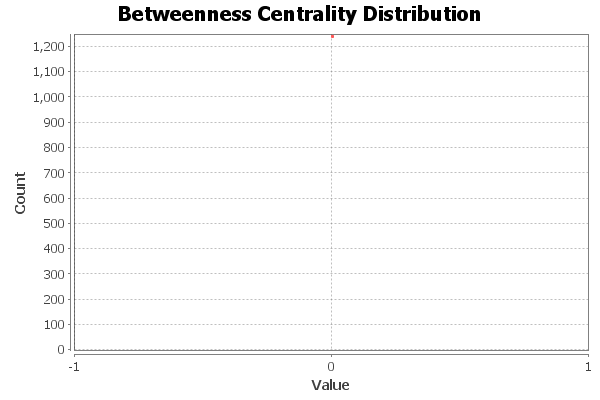
\includegraphics[scale=.5]{BetweennessCentralityDistribution.png}
\end{figure}
\begin{figure}
  \centering
  \caption{Eccentricity distribution}
  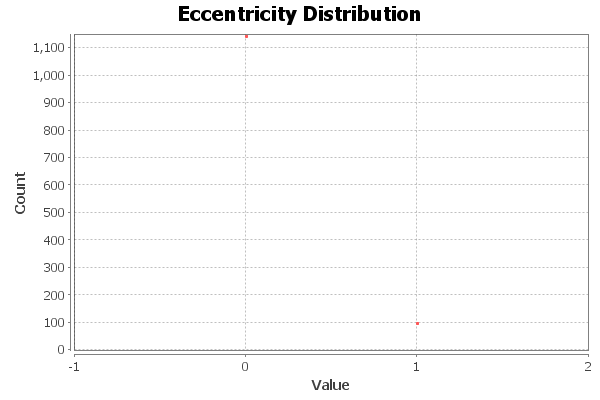
\includegraphics[scale=.5]{EccentricityDistribution.png}
\end{figure}
\graphicspath{{q3/hits/}}
\begin{figure}
  \centering
  \caption{HITS authorities}
  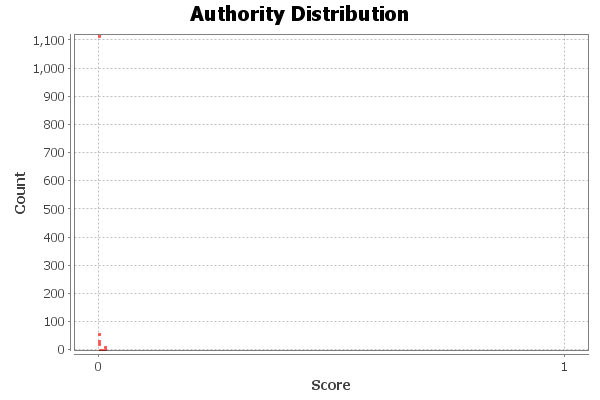
\includegraphics[scale=.5]{authorities.png}
\end{figure}
\begin{figure}
  \centering
  \caption{HITS hubs}
  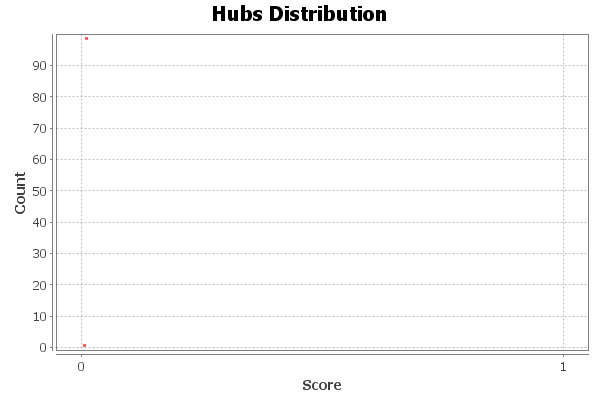
\includegraphics[scale=.5]{hubs.png}
\end{figure}
\graphicspath{{q3/pagerank/}}
\begin{figure}
  \centering
  \caption{Pagerank}
  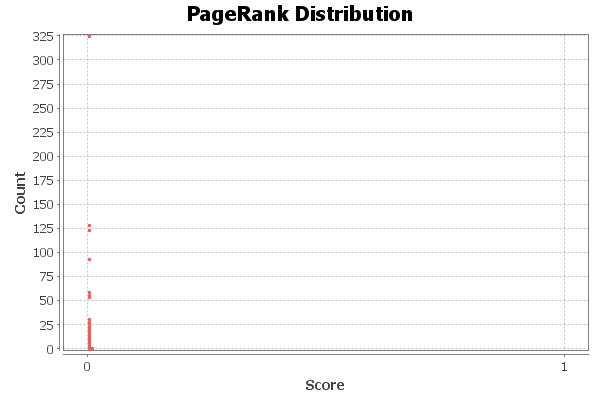
\includegraphics[scale=.5]{pageranks.png}
\end{figure}
\vfill
\clearpage

\newpage
\appendix
Appendix A
\lstinputlisting[language=python]{q1/createLink.py}

\newpage
Appendix B
\lstinputlisting[language=python]{q2/createGraph.py}

\newpage
Appendix C
\lstinputlisting[language=R]{q2/graph.dot}

\end{document} 
